\chapter{Introduction}

\section{Motivation}
Revealing the structure of hierarchical organized data is a complex task where many approaches already exists (TODO cite). It is still an active research area as data scientists are facing ever greater challenges when analyzing large hierarchical datasets. One example is the Human Disease Network \cite{zhou_human_2014} which is a hierarchical network of disorders and disease genes with approximately 3000 nodes on two different hierarchy layers. Figure \ref{fig:Human_Disease_Network} shows us the representation of the data in a common two-dimensional layout. In this representation, the classes of disorders are coded by color. 
Another dataset with a similar structure can be seen in Figure \ref{fig:original2DdiseaseNet}, here the clusters of different diseases are grouped by boxes. Depiction of hierarchical network structure in 2D faces us with many challenges for example: 
\begin{itemize}
    \item \textbf{Limitation of visual features.} Figure \ref{fig:Human_Disease_Network} already uses the color to encode the group membership thus we can not use a color scale to visualize additional attributes like mortality rate.
    \item \textbf{Lack of space.} A common problem in network visualization is the hairball effect, with only two dimensions the reduced space quickly leads to overlapping of nodes and links. In Figure \ref{fig:Human_Disease_Network} we can see this effect on the green nodes. The graph in Figure \ref{fig:original2DdiseaseNet} solves this problem by hiding links between child nodes from different boxes which is also not optimal.
    %\item \textbf{Restriction of cluster detection.} With only two available axes and therefore only two spatial encoded data attributes task like cluster detection and conformation are harder.
\end{itemize} 

\begin{figure}[h]
    \centering
    \begin{subfigure}[b]{0.4\columnwidth}
        \centering
        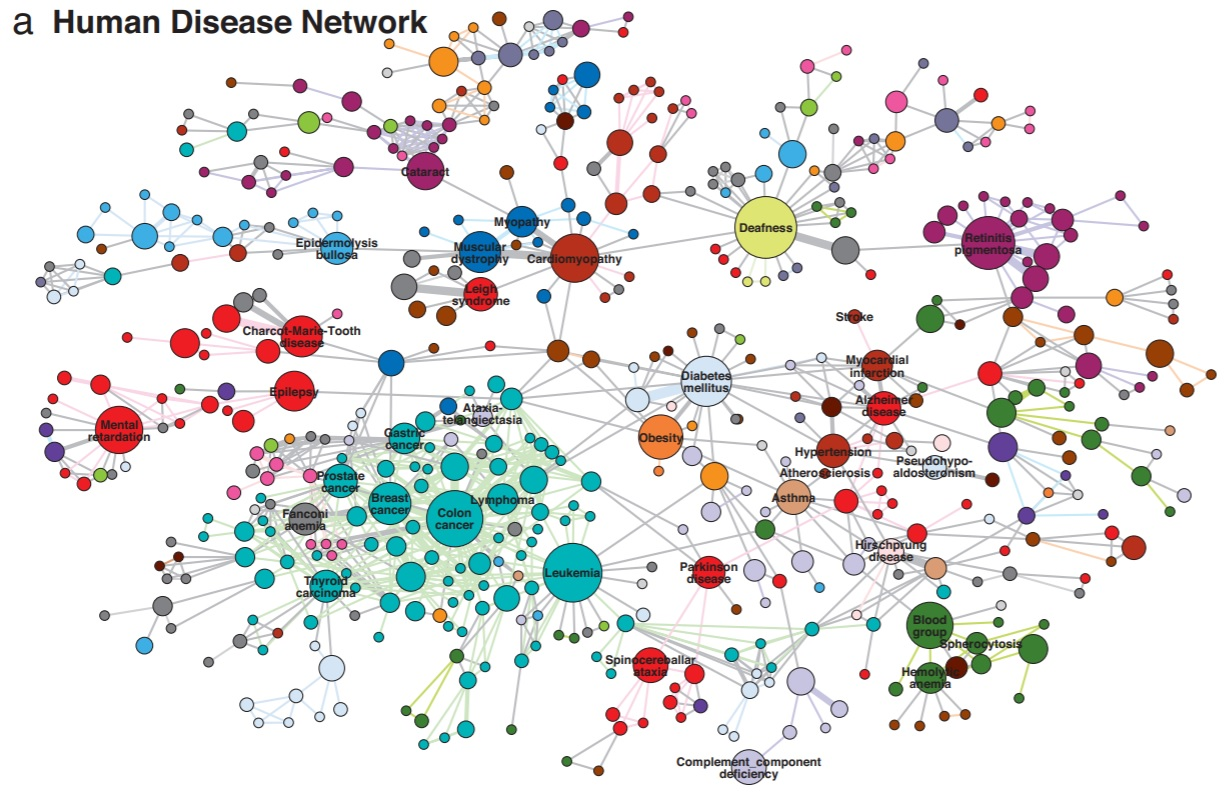
\includegraphics[width=\textwidth, trim={0 0 9cm 0},clip]{graphics/Human_Disease_Network.jpg}
        \subcaption{Human Disease Network \cite{zhou_human_2014}}
        \label{fig:Human_Disease_Network}
    \end{subfigure}
    \begin{subfigure}[b]{0.5\columnwidth}
      \centering
      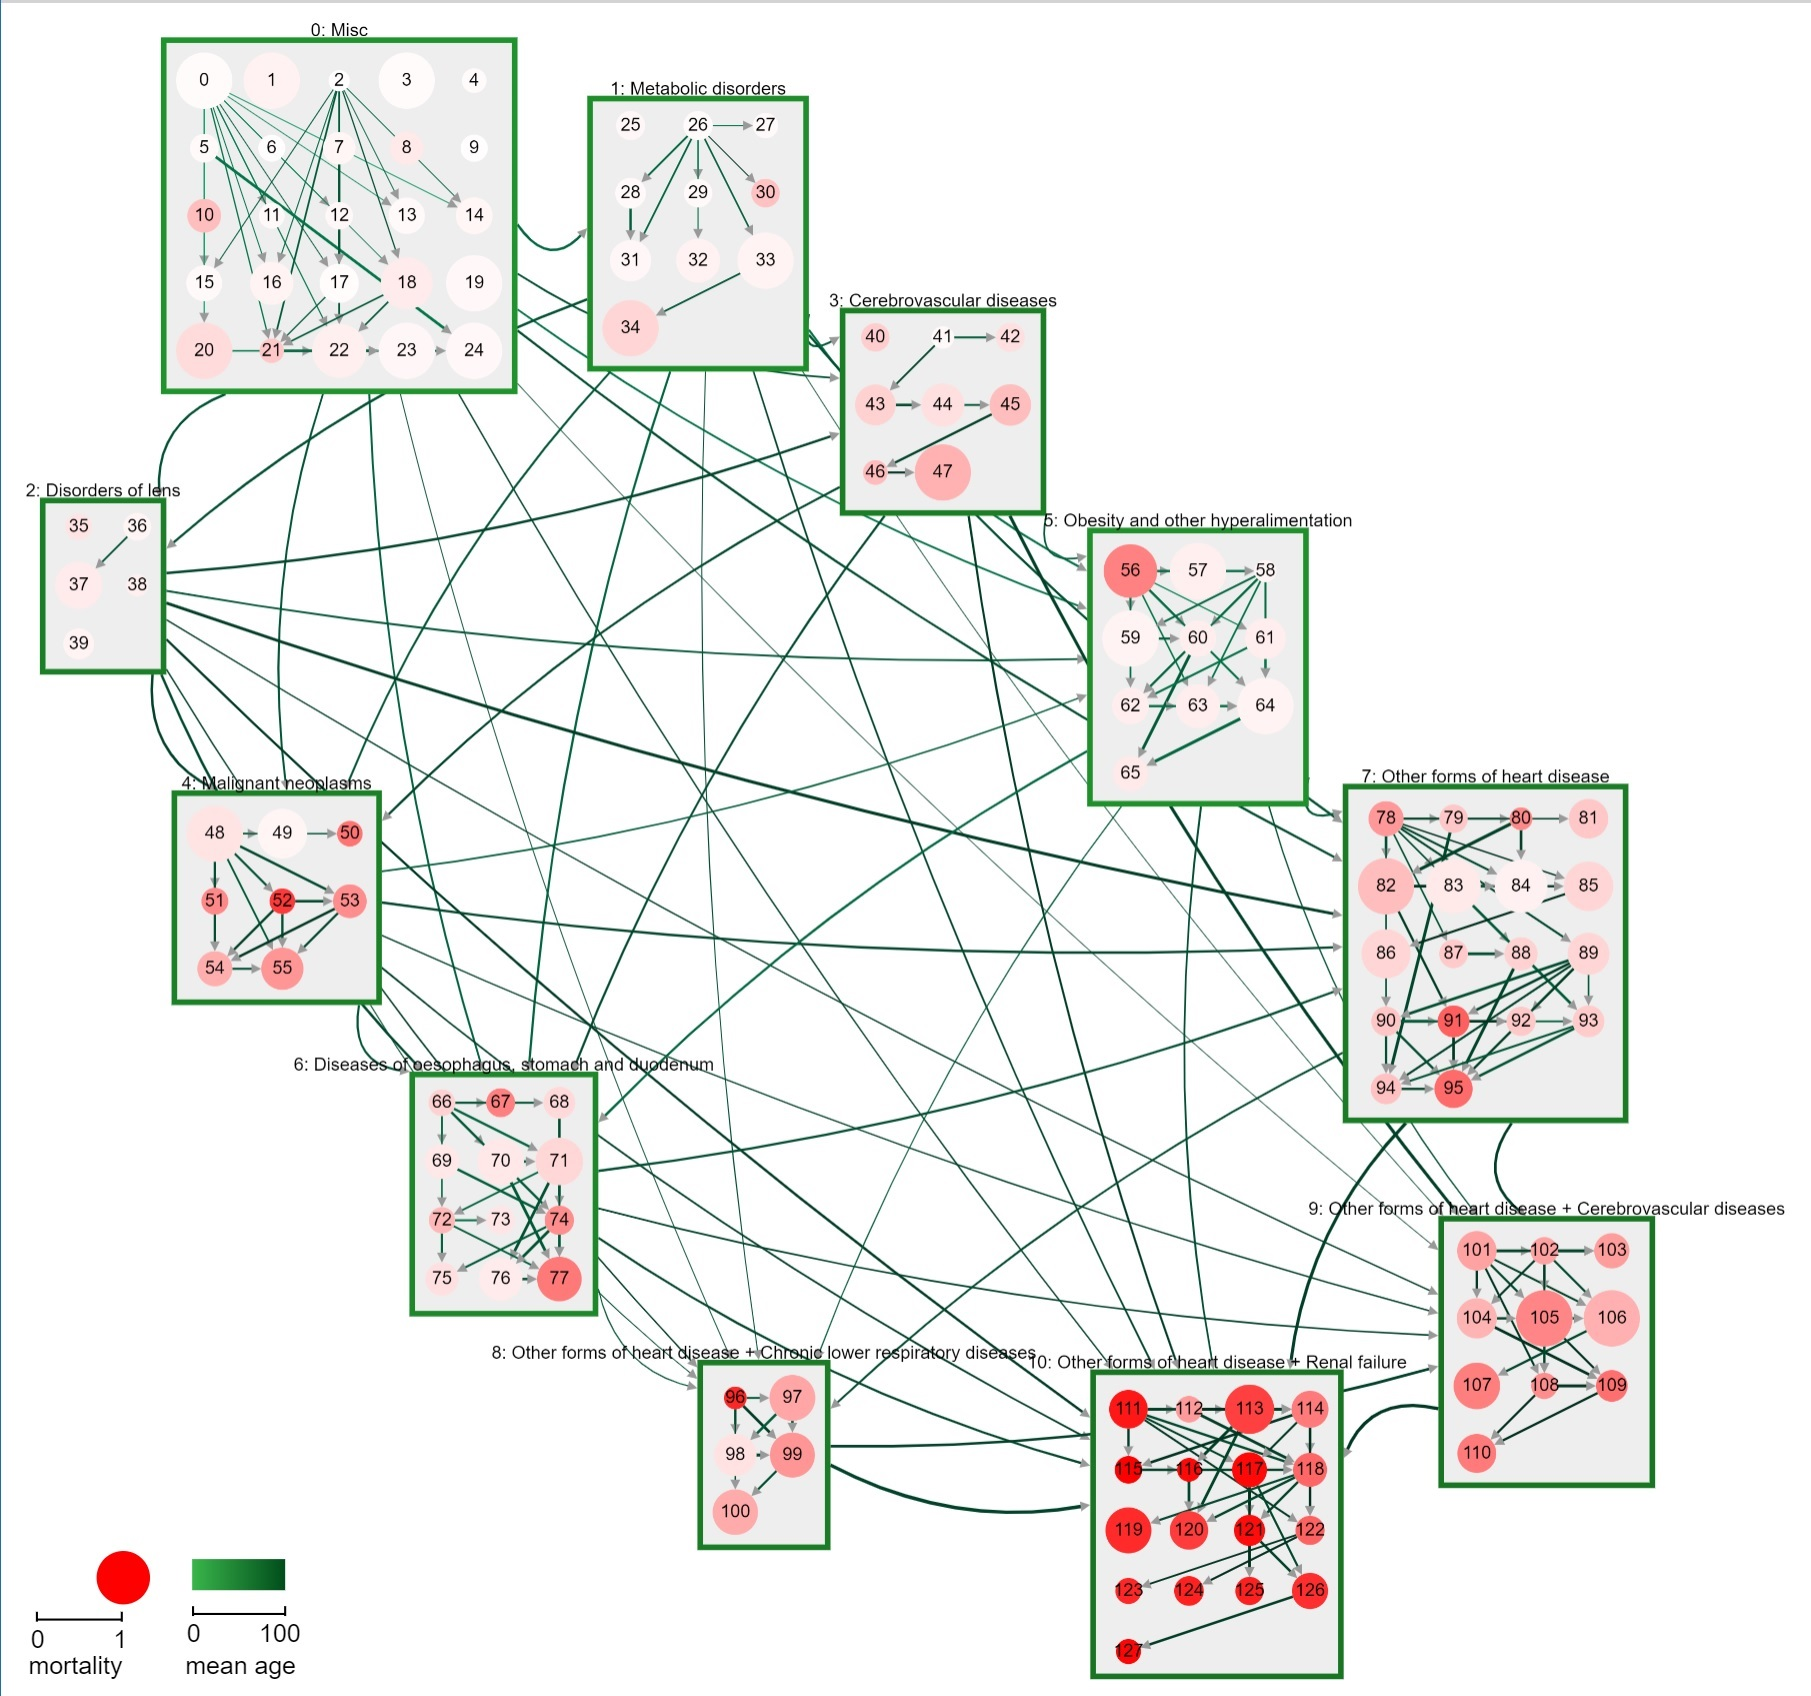
\includegraphics[width=\textwidth]{graphics/original2DdiseaseNet.jpg}
      \subcaption{a comorbidity network of diagnoses related to diabetes melitus}
      \label{fig:original2DdiseaseNet}
    \end{subfigure}
    \caption[Optional caption for the figure list (often used to abbreviate long captions)]{Example visualizations of hierarchical network datasets in two dimensions. Both consists of two hierarchical layers.} % Remove the [...] argument if the original caption should be used in the figure list.
    \label{fig:intro} 
  \end{figure}

3D information visualization allows us to expand the user experience of traditional 2D graphs. As Brath describes in his paper \cite{brath_3d_2014} there are many advantages and opportunities when using three-dimensional visualizations.
%The additional axes allow us to encode an additional attribute by its position, this can be seen in the “3D space time cube” \cite{brath_3d_2014} here the temporal information is encoded on the Z axis another common usage is a 3D scatter plot. 
By using an additional axis the visualization has more space to distribute all the data and reduce clutter in the first place before applying specialized layouts. The mental model of the data gets improved which leads to a better cluster detection, conformation and general overview of the data.
In the context of visual features, we get a lot more of opportunities, for example the ability to use surfaces and effects like shading. 
In three-dimensional layouts, the perspective of the visualization has to be reconsidered. Usually the user looks from the outside with a bird's eye view at the visualization. In 3D however the viewer can be placed right inside our graph, this enables us to utilize new navigation and interaction possibilities. Some visualization also use the additional axis to encode an extra attribute by its position, this can be seen in the “3D space time cube” \cite{brath_3d_2014} here the temporal information is encoded on the Z axis another common usage is a 3D scatter plot. 

Still, all these opportunities also involve new challenges: navigation inside the visualization, occlusion of elements in an 3D perspective view, selection of objects for displaying details and the lack of a reference point in three-dimensional space. Brath \cite{brath_3d_2014} already stated that immersive interfaces could help to overcome this issues.
 We believe that with the recent developments in virtual reality hardware and frameworks these challenges can now be addressed even better. 
 We can see the benefits of VR based visualizations in various publications. Bowman et al. \cite{bowman_virtual_2007} examined the impact of VR techniques, like stereoscopic images, interaction with the virtual world and head movement, can have on users. 
 Recently Kraus et al. \cite{kraus_impact_2020} did a study on the effect of immersion for detecting clusters in a scatter plot. Their results show that VR based visualization systems have real world advantages in terms of time needed to get an overview of the data compared to traditional 2D- and 3D information visualization. 
 
\section{Aim of the Work}

Our goal is to implement a visualization for hierarchical network data that allows users take the benefits of 3D information visualization and opportunities of virtual reality technology to dive right into the data. We believe the combination of both concepts complete each other well because VR based technology can be used to solve the subsequent challenges from 3D information visualization and therefore enable data scientists to optimize their data analysis tasks. 
To this end, we designed a customized graph layout (see Figure \ref{fig:conceptSketch}).
This calculates the position and size of each node by the hierarchical structure: child nodes are nested within its parent node. In addition, it takes care of preventing visual clutter by overlapping of nodes and links. 
Furthermore, the exploration of the resulting graph should be possible with room scaled virtual reality devices like the HTC Vive. So we implemented VR optimized navigation, filtering and brushing methods to enhance the graph exploration user experience. 
To evaluate our results we gathered feedback from multiple people including ourselves on overview of the visualization, navigation, interaction and motion sickness. However, a full user study is out of scope of this thesis.

\section{Methodology}
As stated by Sadana et al. \cite{sadana_redefining_2016}, it is also important to explore how existing techniques can be applied to new platforms like virtual reality devices. To this end, we take existing already well established 2D visualization techniques combine them and extend the result into the three-dimensional space. We adapted a tree map visualization (see Figure \ref{fig:hierarchicalCirclePlot}) for visualizing the hierarchical aspect and a flat multilayer network (see Figure \ref{fig:2dmultilayerVis}) for the network relationships.  

Our core concepts are the following: 
\begin{itemize}
    \item We render each hierarchy layer as a three-dimensional structure instead a flat surface as seen in most multilayer network visualizations. This enables us to use the whole volume to evenly distribute our nodes and links of the network. Thereby reducing the edge and node-edge crossings in comparison to a flat surface.   
    \item For the hierarchical relationship, we use the concept of nesting child nodes into parent nodes as seen in tree map visualizations. However, we use 3D spheres instead of 2D boxes. 
    \item Links between nodes are possible in one network but also to other networks of the same hierarchical layer. The visibility of the links is changed automatically and manually during the exploration process. 
    \item For user input we fully utilize the tracking capabilities of the HTC Vive controllers. Selection of nodes and links is possible with a virtual “laser pointer” attached to the user's controller in the scene.
    \item For navigation, we provide two kinds of navigation methods: One for bridging larger distances like flying to a specific node selected by the user or flying to the hierarchical parent node. Additional, a free flying navigation that allows the user to fine tune their position.
    \item We dynamically adjust the size of the entire scene while exploring the graph. This is necessary as in a virtual reality scene the size of objects is always directly linked to real world sizes. (e.g. 1 virtual unit is 1 meter in the players VR setup)
\end{itemize}
The result can be seen in Figure \ref{fig:conceptSketch}.
In addition, our visualization is not limited to two hierarchical layers as seen in the Figure, but rather is able to display $n$ hierarchical layers. To achieve this we simply repeat the process of nesting child nodes into parents for each layer.

\begin{figure}[h]
    \centering
    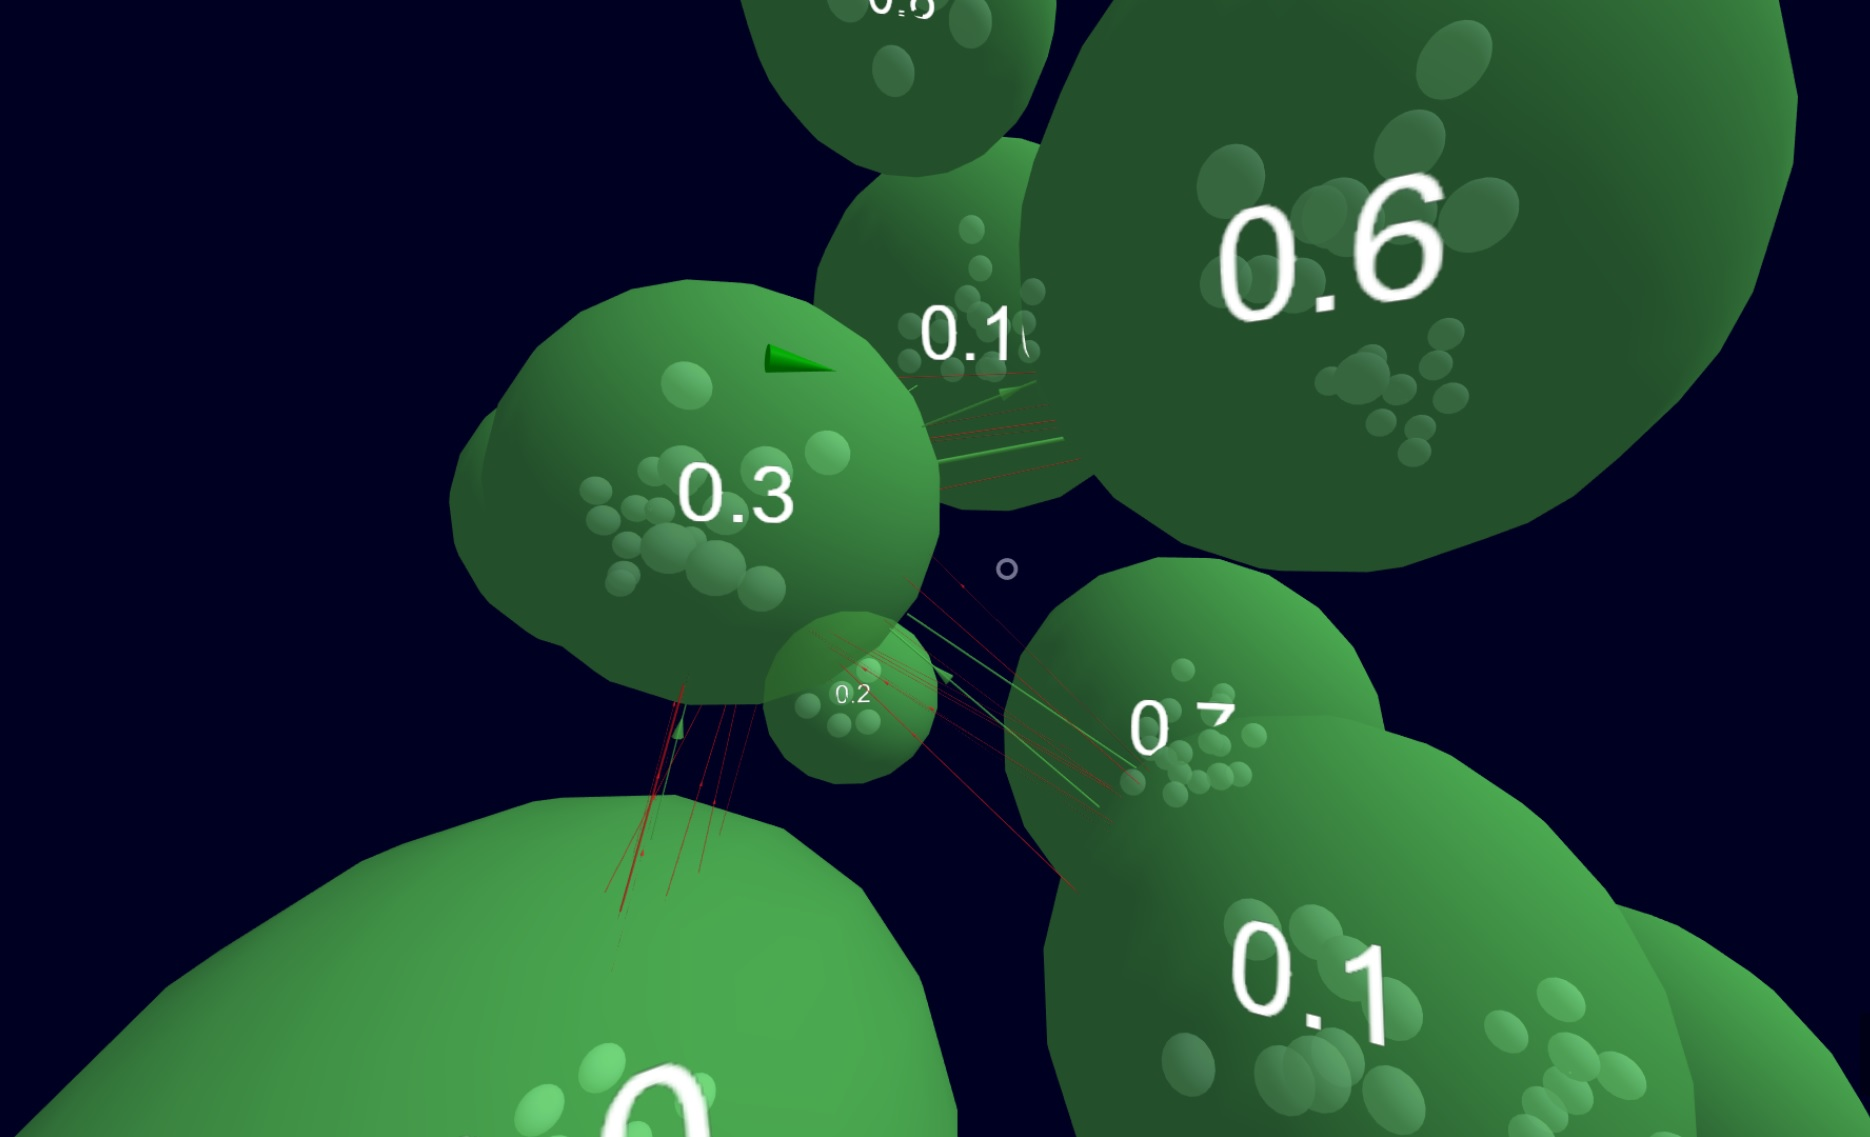
\includegraphics[width=1\textwidth]{graphics/conceptScreenshot.jpg}
    \caption{Screenshot of the comorbidity network dataset from \ref{fig:original2DdiseaseNet} in our hierarchical network visualization. On the screenshot only edges from node 0.3 are displayed.} % Remove the [...] argument if the original caption should be used in the figure list.
    \label{fig:conceptSketch} 
\end{figure}
